\begin{frame}
    \frametitle{Basis sets in chemistry}
    \vspace{1.8mm}
    \begin{columns}
    \begin{column}{.10\textwidth}
    \end{column}
    \begin{column}{.30\textwidth}
    \textbf{Attractive features}
    \begin{itemize}
        \item Precision
        \item Compactness
        \item Efficiency
        \item Systematicity
        \item Universality
    \end{itemize}
    \end{column}
    \begin{column}{.60\textwidth}

    \vspace{5mm}

    \end{column}
    \end{columns}

    \vspace{40.2mm}

\end{frame}

\begin{frame}
    \frametitle{Basis sets in chemistry}
    \begin{columns}
    \begin{column}{.10\textwidth}
    \end{column}
    \begin{column}{.30\textwidth}
    \textbf{Attractive features}
    \begin{itemize}
        \item {\color{green} Precision}
        \item {\color{green} Compactness}
        \item {\color{red} Efficiency}
        \item {\color{yellow} Systematicity}
        \item {\color{yellow} Universality}
    \end{itemize}
    \end{column}
    \begin{column}{.60\textwidth}
    \centering
    \textbf{Atoms-centered basis sets}
    \begin{equation}
        \nonumber
        \chi(\rvec) = R(r)Y_{lm}(\theta,\varphi)
    \end{equation}

    \vspace{5mm}

    \textbf{Slater-type orbitals}
    \begin{equation}
        \nonumber
        R^{STO}(r) \propto e^{-\zeta r}
    \end{equation}
    \end{column}
    \end{columns}

    \vspace{5mm}

    \begin{center}
    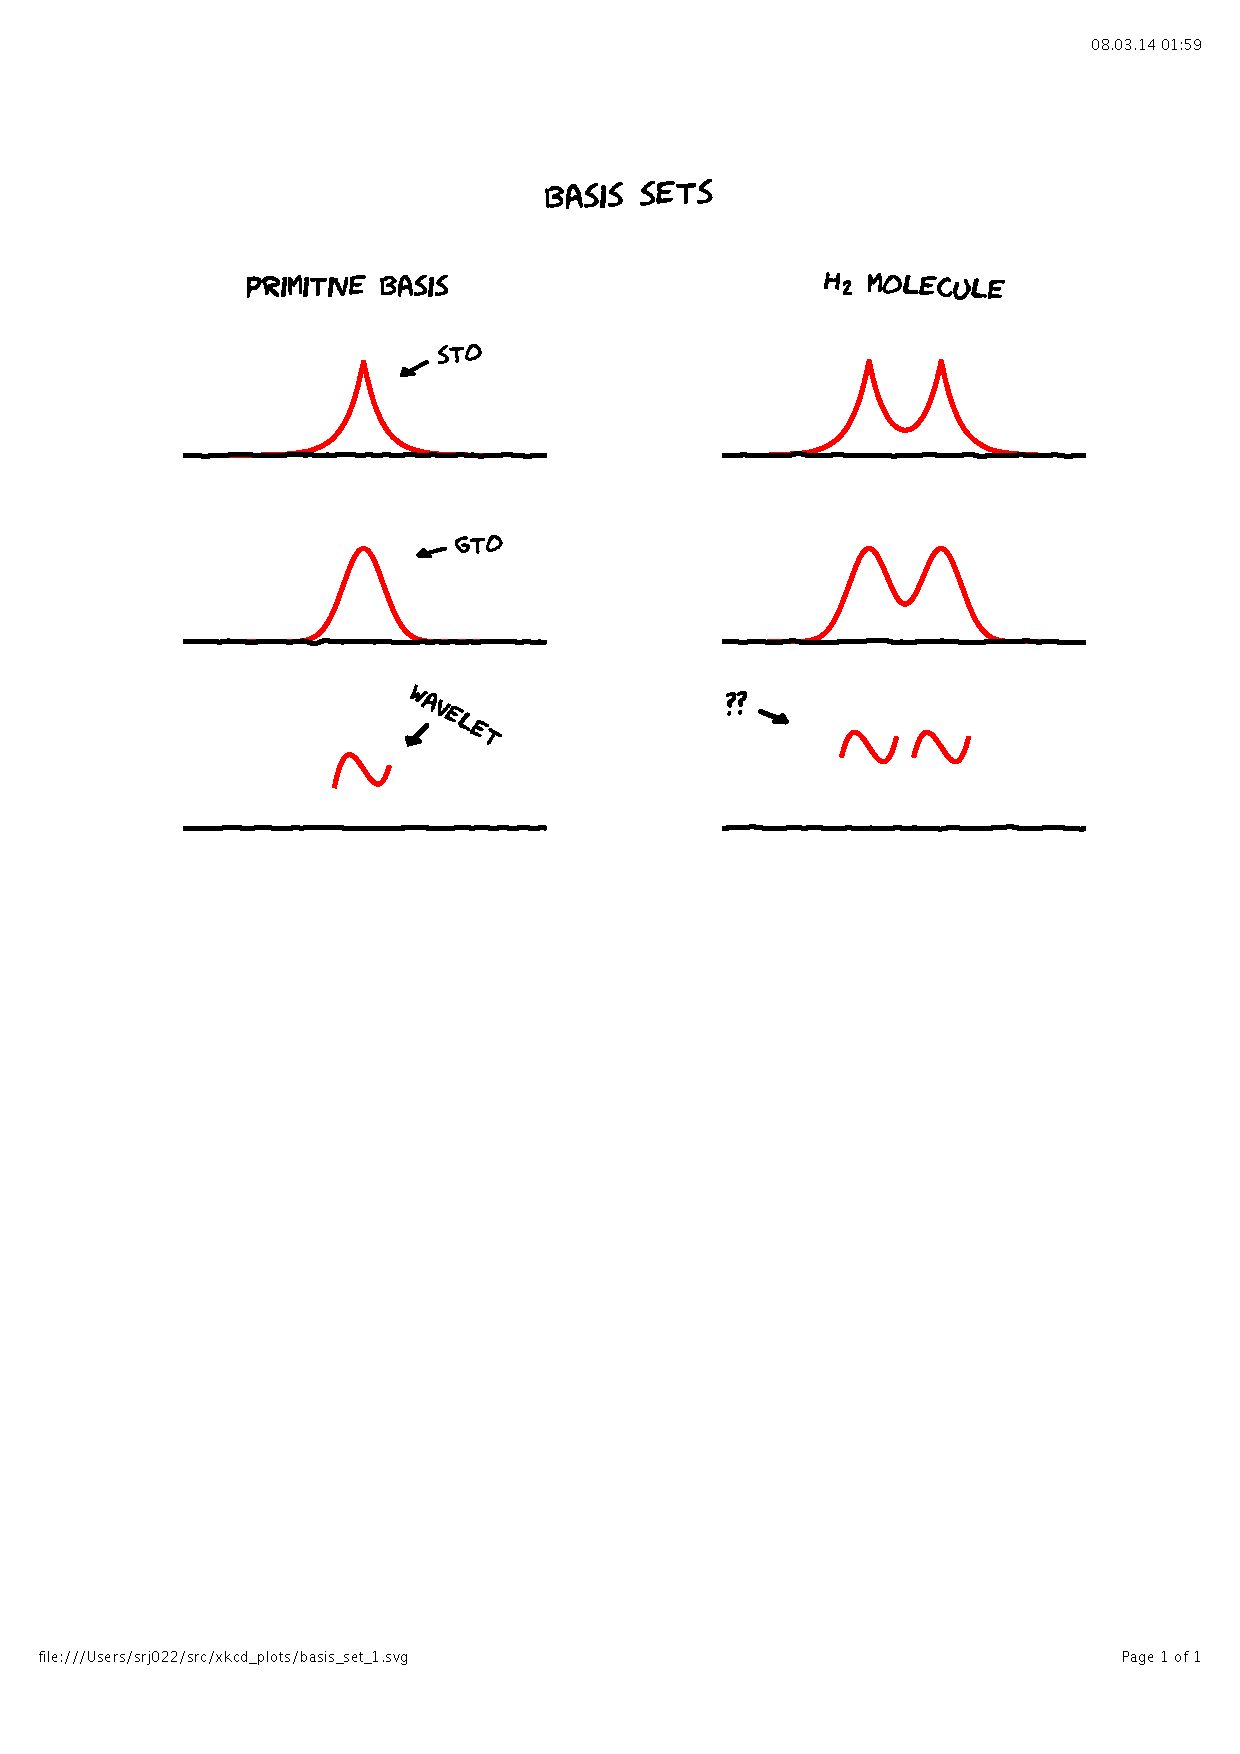
\includegraphics[scale=0.6, clip, viewport = 50 680 550 730]{figures/basis_set_1.pdf}\\
    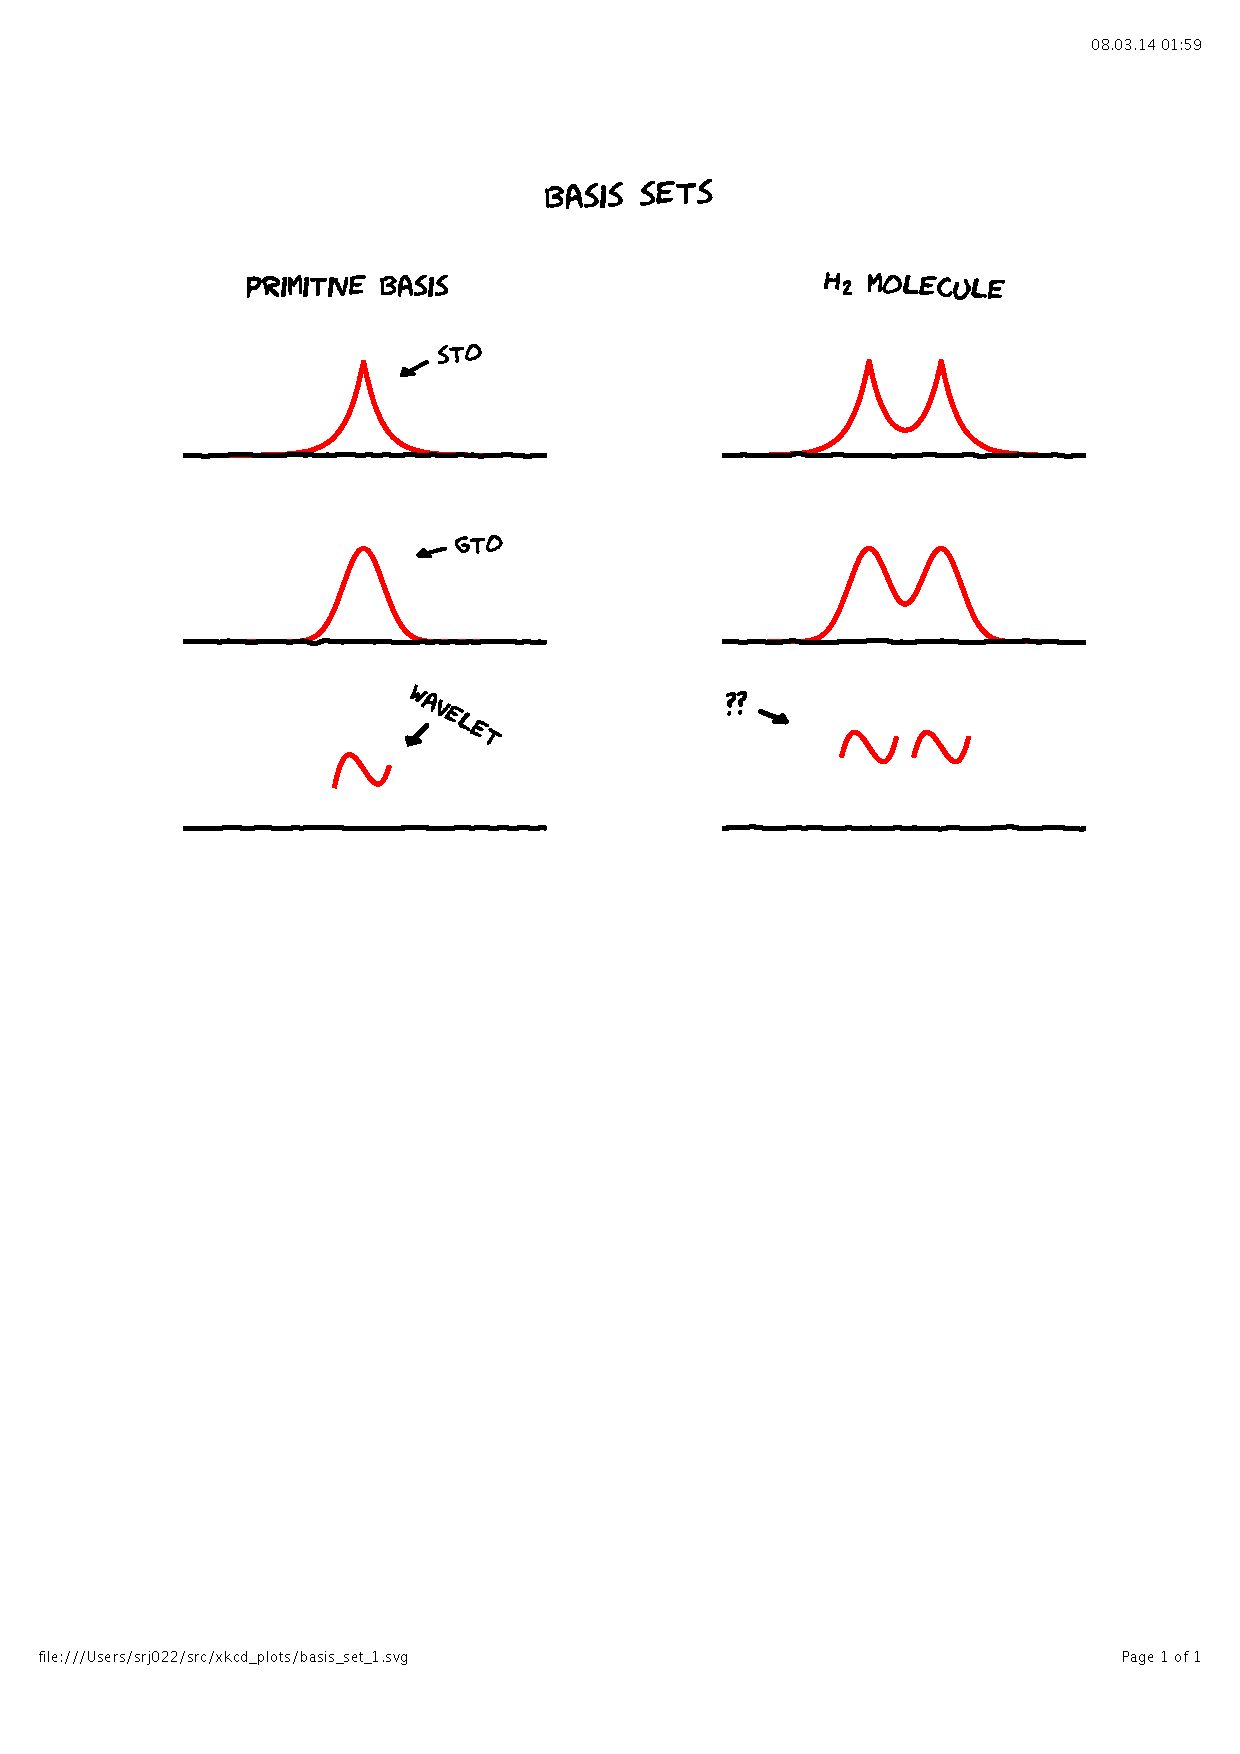
\includegraphics[scale=0.6, clip, viewport = 50 615 550 695]{figures/basis_set_1.pdf}
    \end{center}
\end{frame}

\begin{frame}
    \frametitle{Basis sets in chemistry}
    \begin{columns}
    \begin{column}{.10\textwidth}
    \end{column}
    \begin{column}{.30\textwidth}
    \textbf{Attractive features}
    \begin{itemize}
        \item {\color{yellow} Precision}
        \item {\color{yellow} Compactness}
        \item {\color{green} Efficiency}
        \item {\color{yellow} Systematicity}
        \item {\color{red} Universality}
    \end{itemize}
    \end{column}
    \begin{column}{.60\textwidth}
    \centering
    \textbf{Atoms-centered basis sets}
    \begin{equation}
        \nonumber
        \chi(\rvec) = R(r)Y_{lm}(\theta,\varphi)
    \end{equation}

    \vspace{4.2mm}

    \textbf{Gaussian-type orbitals}
    \begin{equation}
        \nonumber
        R^{GTO}(r) \propto e^{-\zeta r^2}
    \end{equation}
    \end{column}
    \end{columns}

    \vspace{5mm}

    \begin{center}
    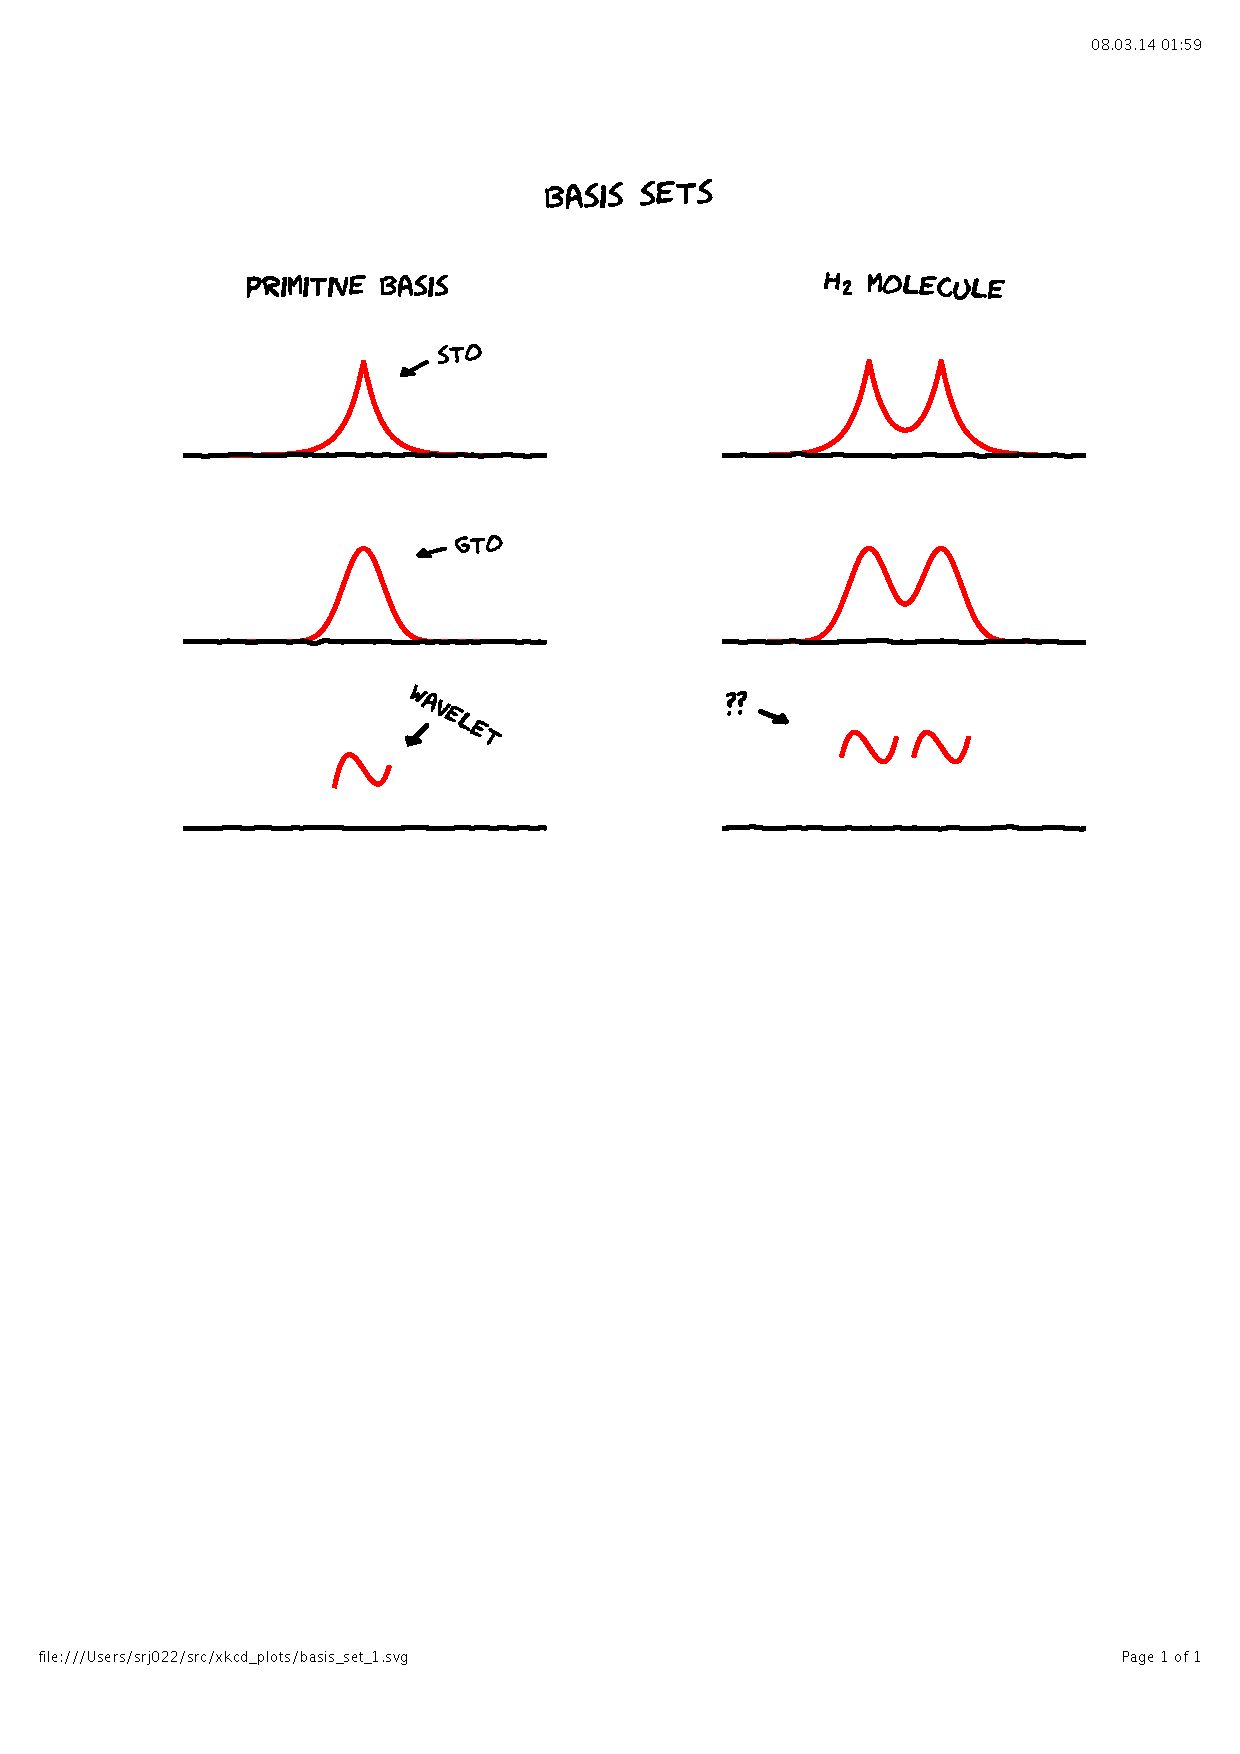
\includegraphics[scale=0.6, clip, viewport = 50 680 550 730]{figures/basis_set_1.pdf}\\
    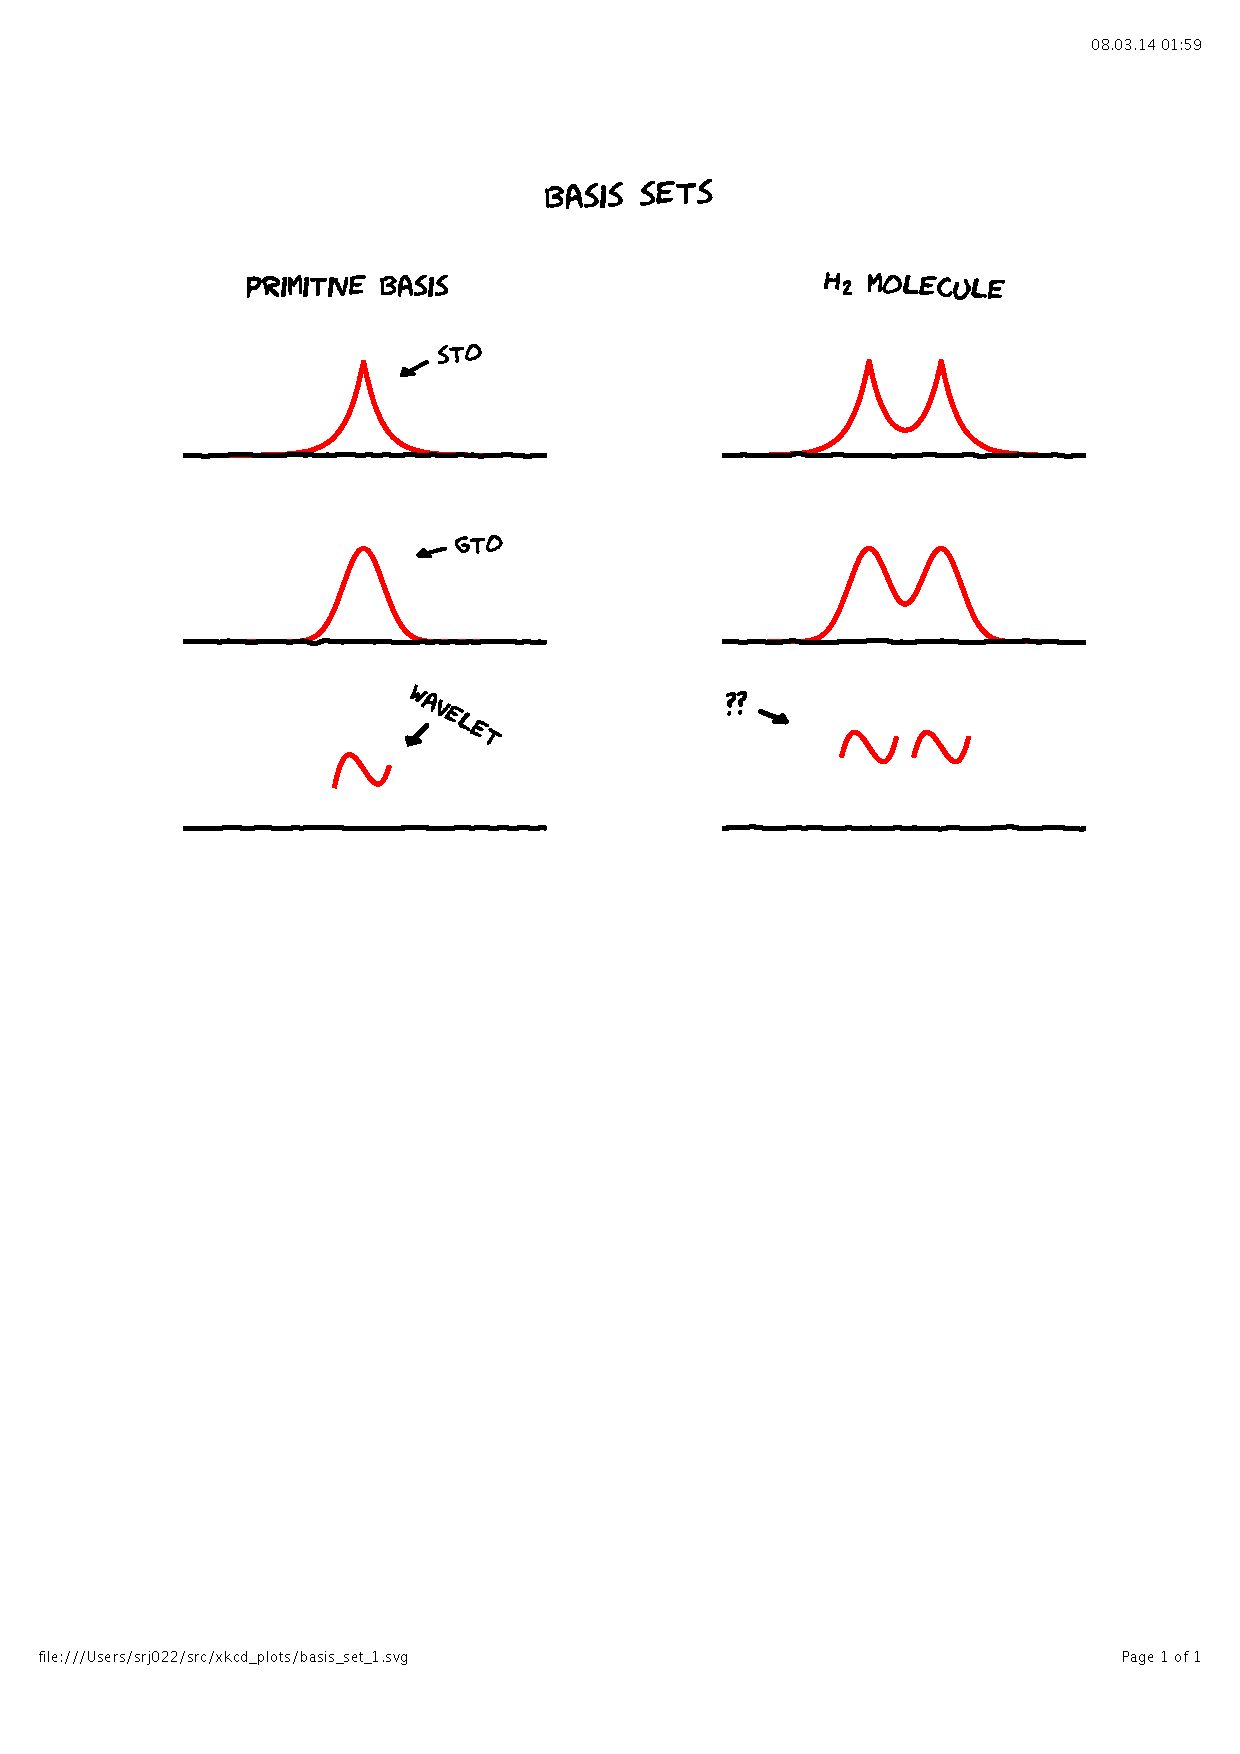
\includegraphics[scale=0.6, clip, viewport = 50 525 550 605]{figures/basis_set_1.pdf}
    \end{center}
\end{frame}

\begin{frame}
    \frametitle{Basis sets in chemistry}
    \begin{columns}
    \begin{column}{.10\textwidth}
    \end{column}
    \begin{column}{.30\textwidth}
    \textbf{Attractive features}
    \begin{itemize}
        \item {\color{yellow} Precision}
        \item {\color{yellow} Compactness}
        \item {\color{green} Efficiency}
        \item {\color{green} Systematicity}
        \item {\color{yellow} Universality}
    \end{itemize}
    \end{column}
    \begin{column}{.60\textwidth}
    \centering
    \textbf{Plane-wave basis sets}
    \begin{equation}
        \nonumber
        \chi(\rvec) = e^{i\bs{k}\cdot\bs{r}}
    \end{equation}
    \end{column}
    \end{columns}

    \vspace{5mm}

    \begin{center}
    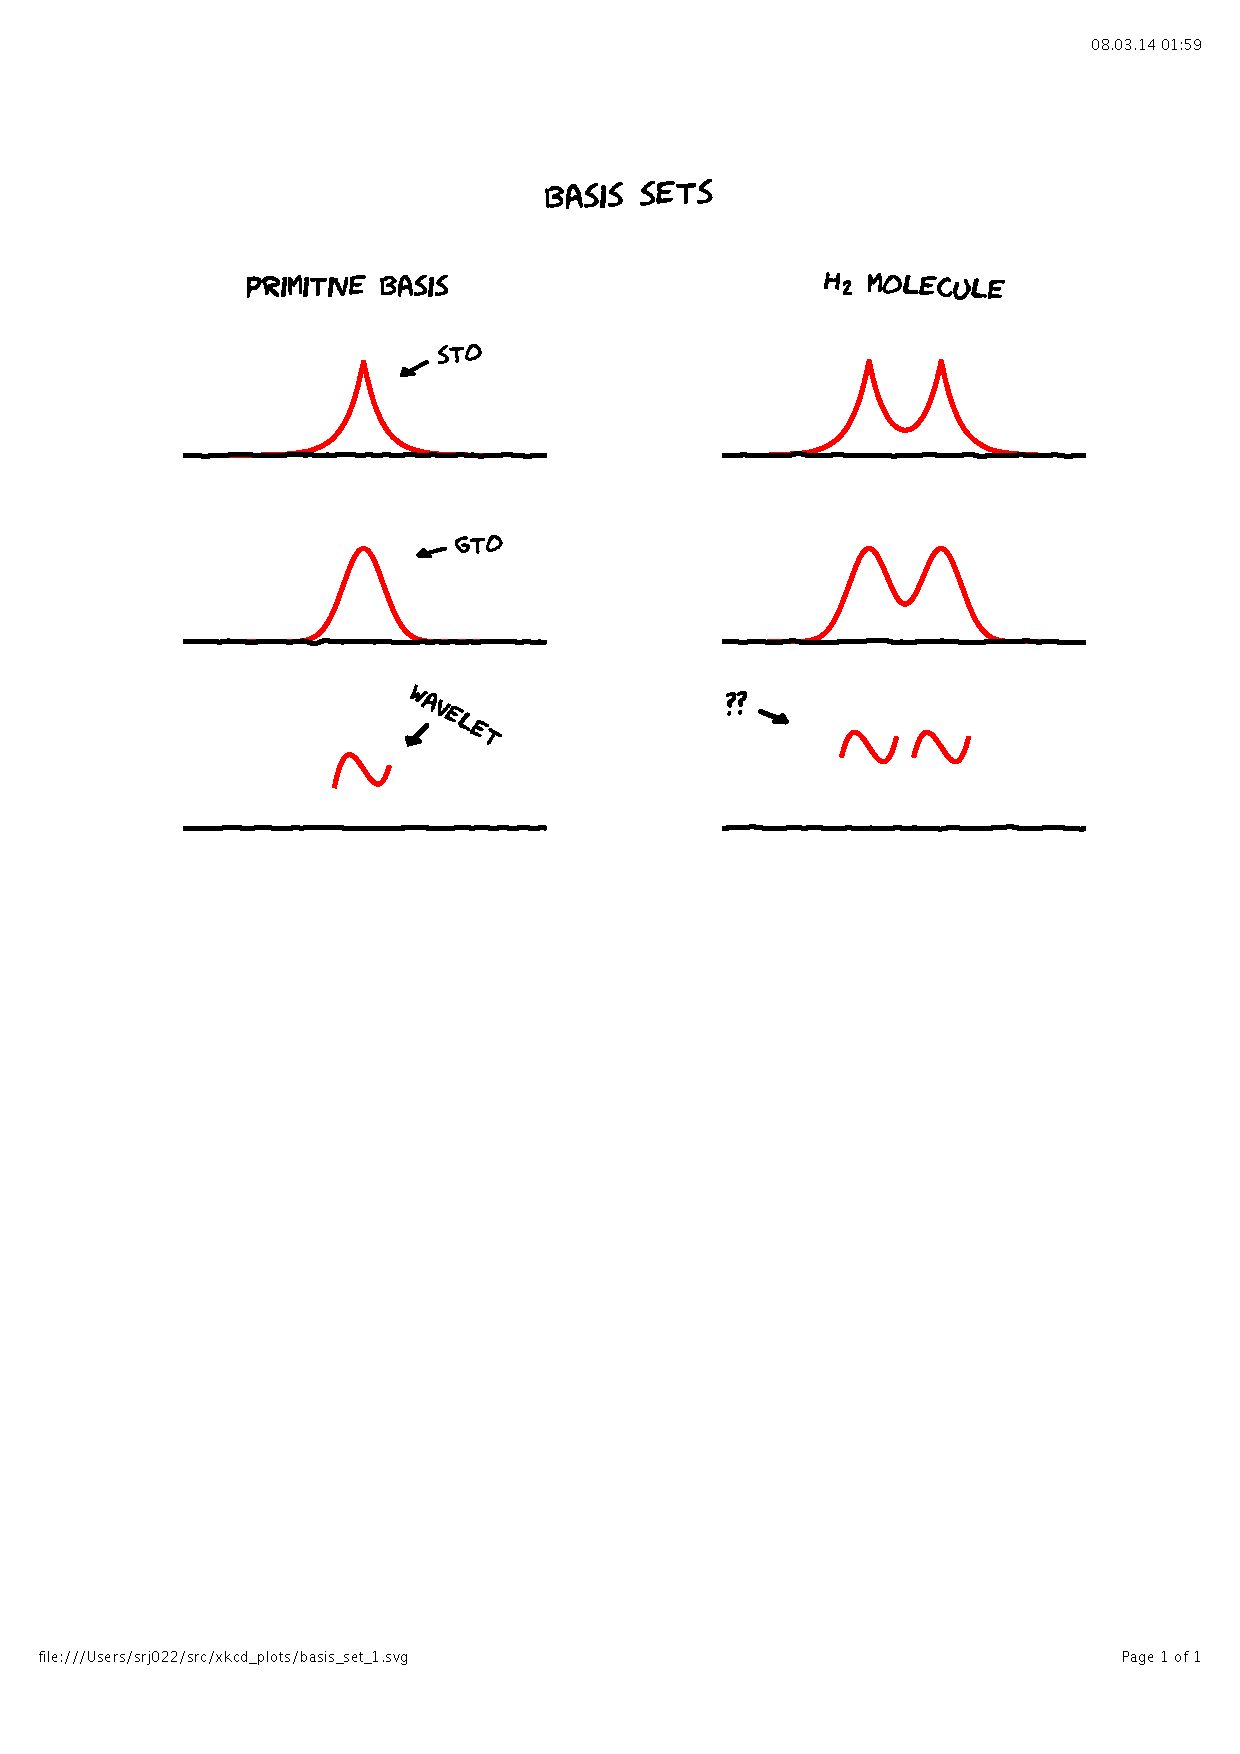
\includegraphics[scale=0.6, clip, viewport = 50 680 550 730]{figures/basis_set_1.pdf}\\
    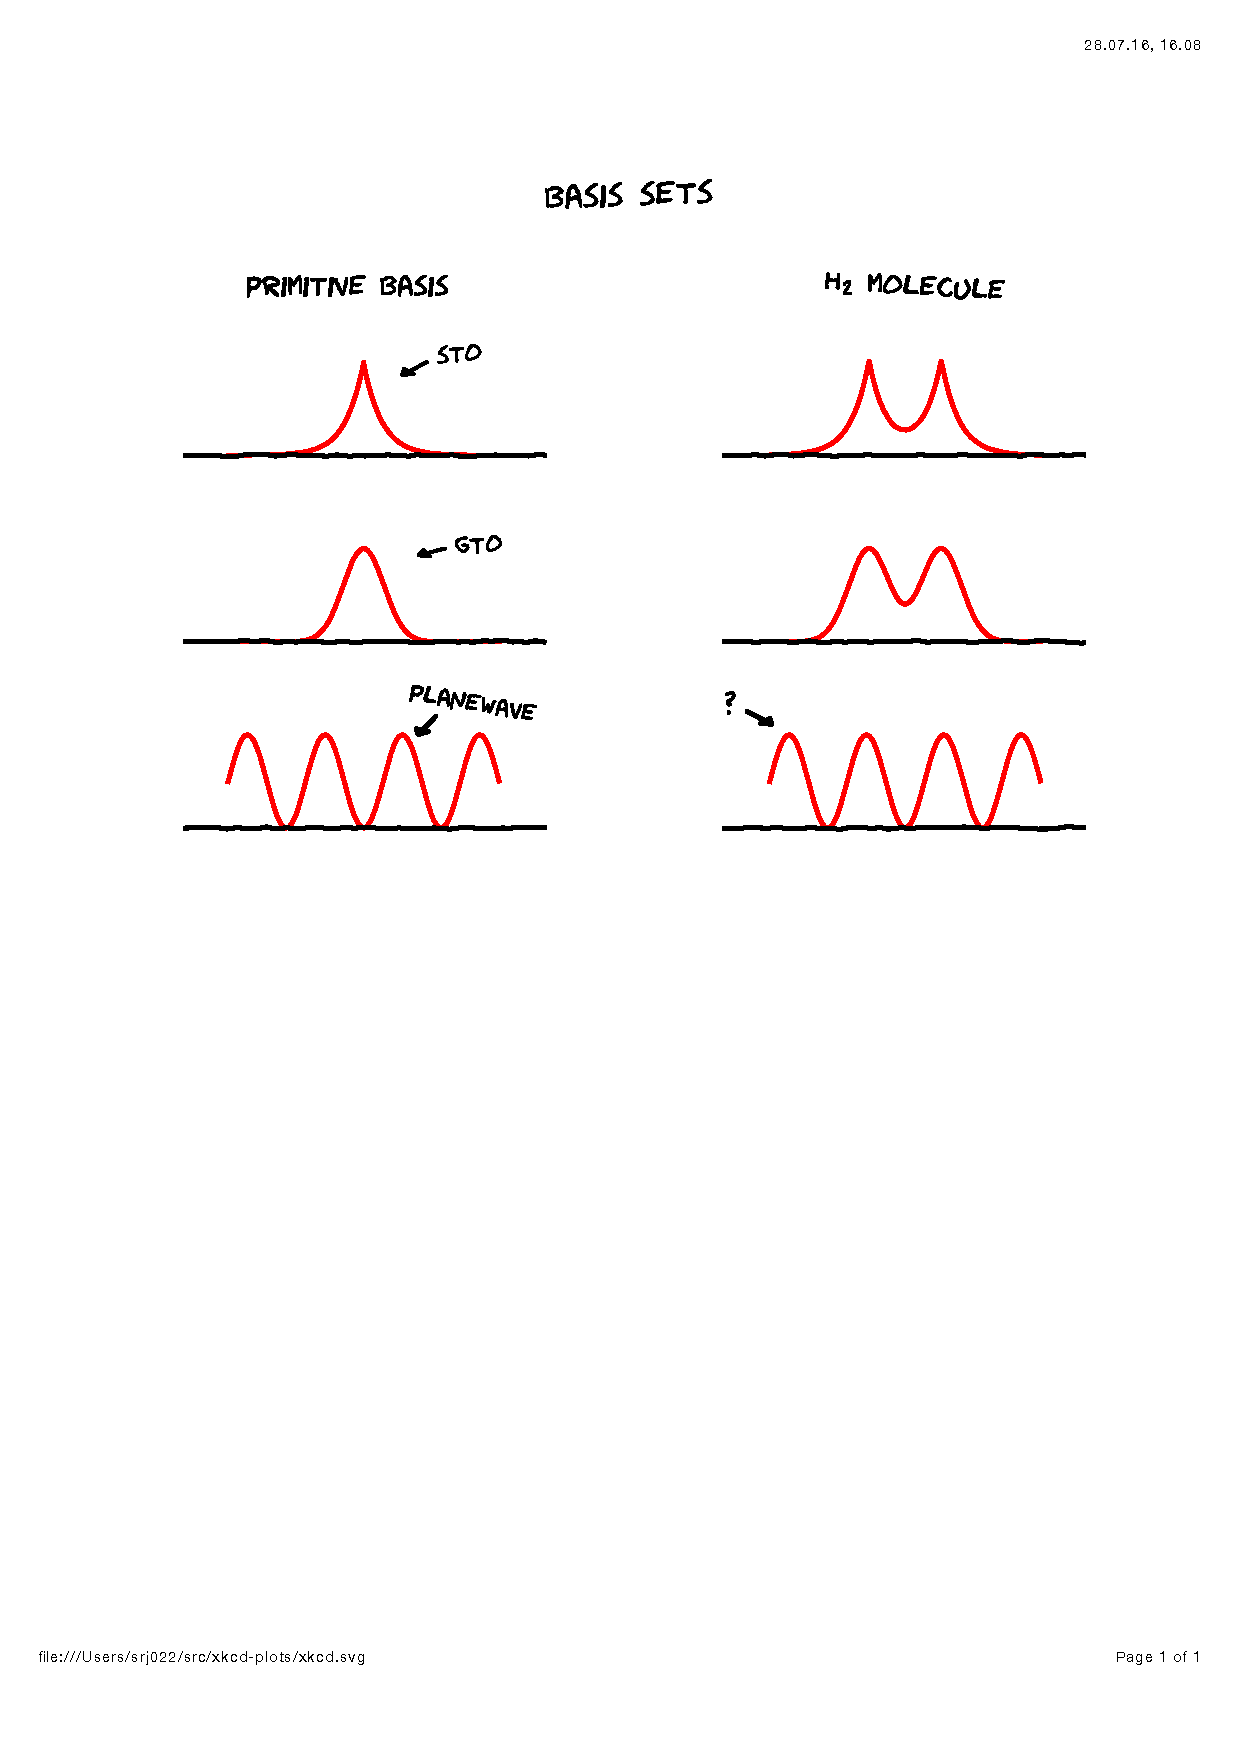
\includegraphics[scale=0.6, clip, viewport = 50 435 550 515]{figures/basis_set_3.pdf}
    \end{center}
\end{frame}

\begin{frame}
    \frametitle{Basis sets in chemistry}
    \begin{columns}
    \begin{column}{.10\textwidth}
    \end{column}
    \begin{column}{.30\textwidth}
    \textbf{Attractive features}
    \begin{itemize}
        \item {\color{green} Precision}
        \item {\color{red} Compactness}
        \item {\color{green} Efficiency}
        \item {\color{green} Systematicity}
        \item {\color{green} Universality}
    \end{itemize}
    \end{column}
    \begin{column}{.60\textwidth}
    \centering
    \textbf{Real-space basis sets}
    \begin{equation}
        \nonumber
        \chi(\rvec) = \phi_i(x)\phi_j(y)\phi_k(z)
    \end{equation}

    \vspace{4.2mm}

    \textbf{Multiwavelets}
    \begin{equation}
        \nonumber
        \phi_{j,l}^n(x) = 2^{n/2}\phi_j(2^nx-l)
    \end{equation}
    \end{column}
    \end{columns}

    \vspace{5mm}

    \begin{center}
    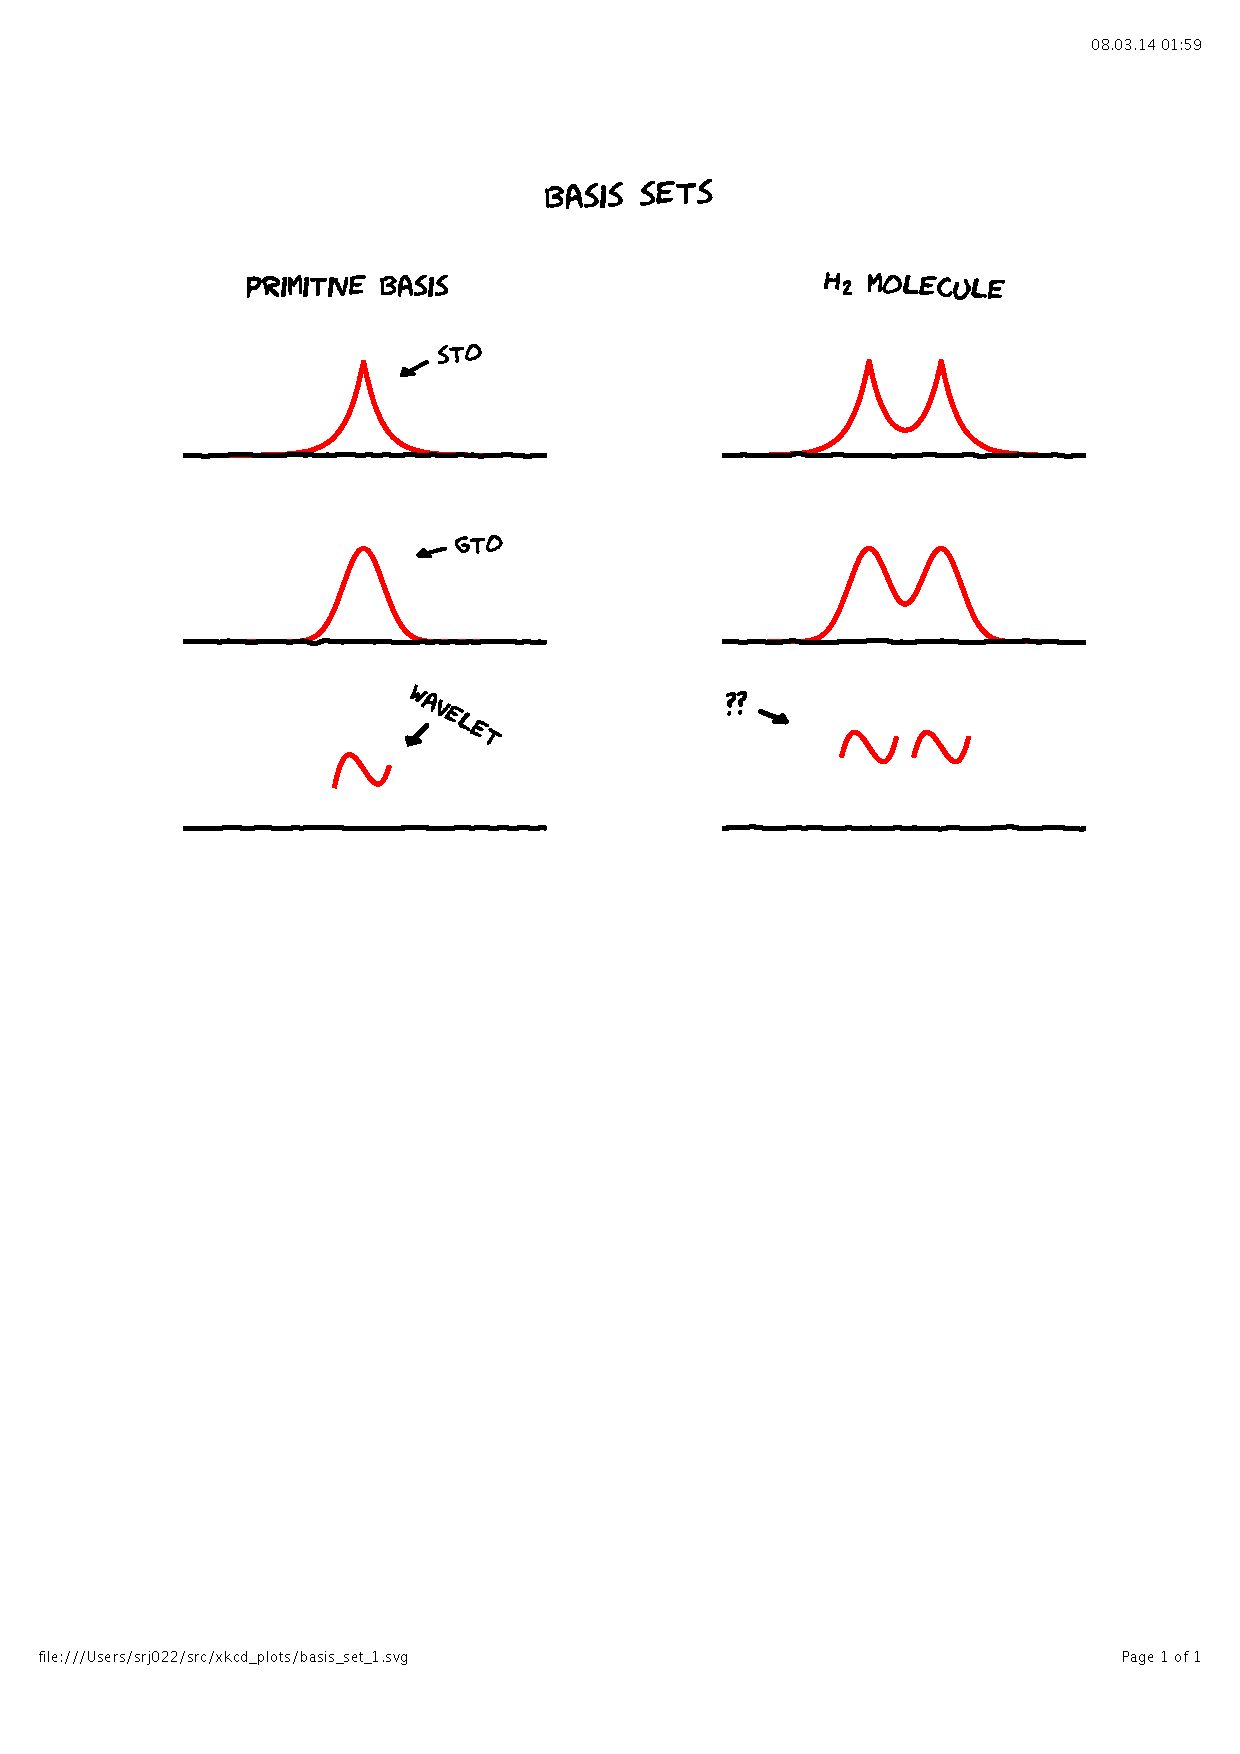
\includegraphics[scale=0.6, clip, viewport = 50 680 550 730]{figures/basis_set_1.pdf}\\
    \only<1>{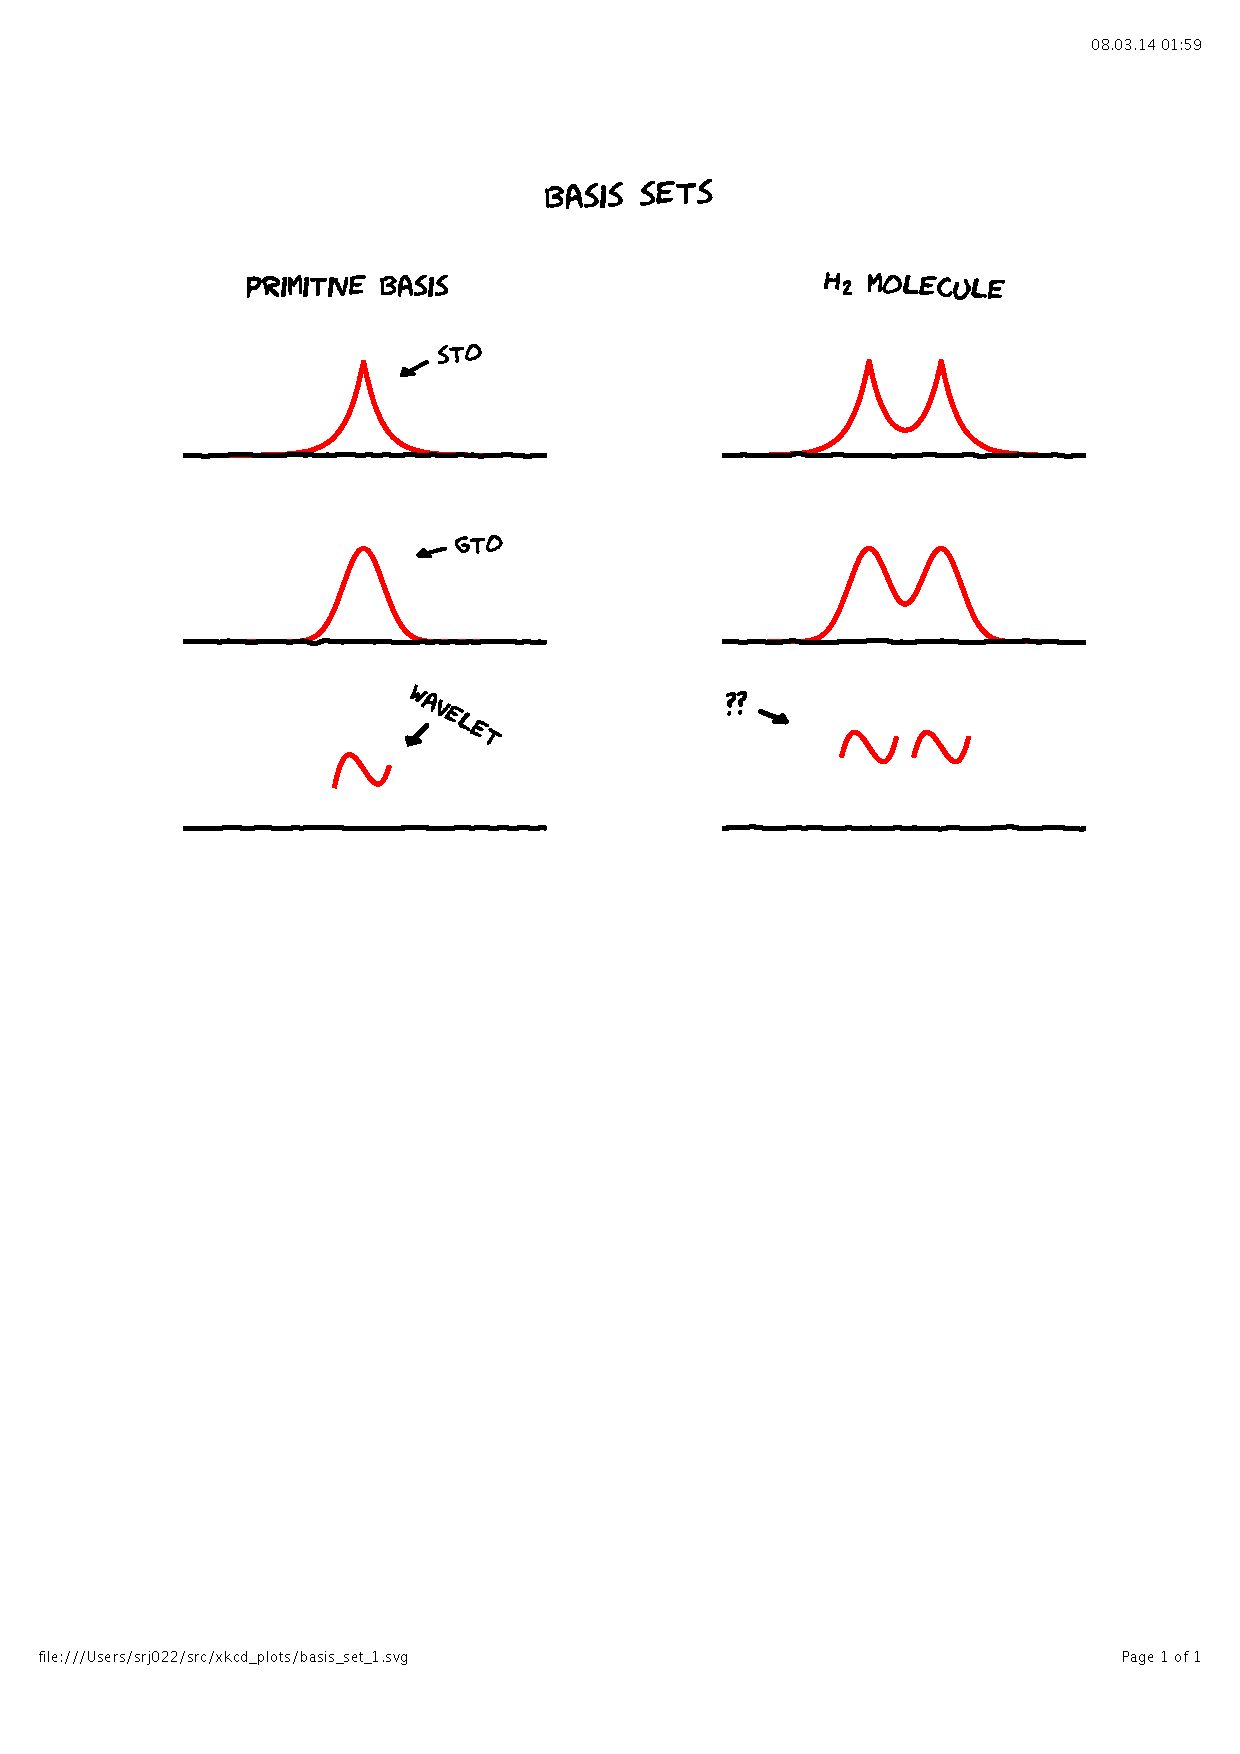
\includegraphics[scale=0.6, clip, viewport = 50 435 550 515]{figures/basis_set_1.pdf}}
    \only<2>{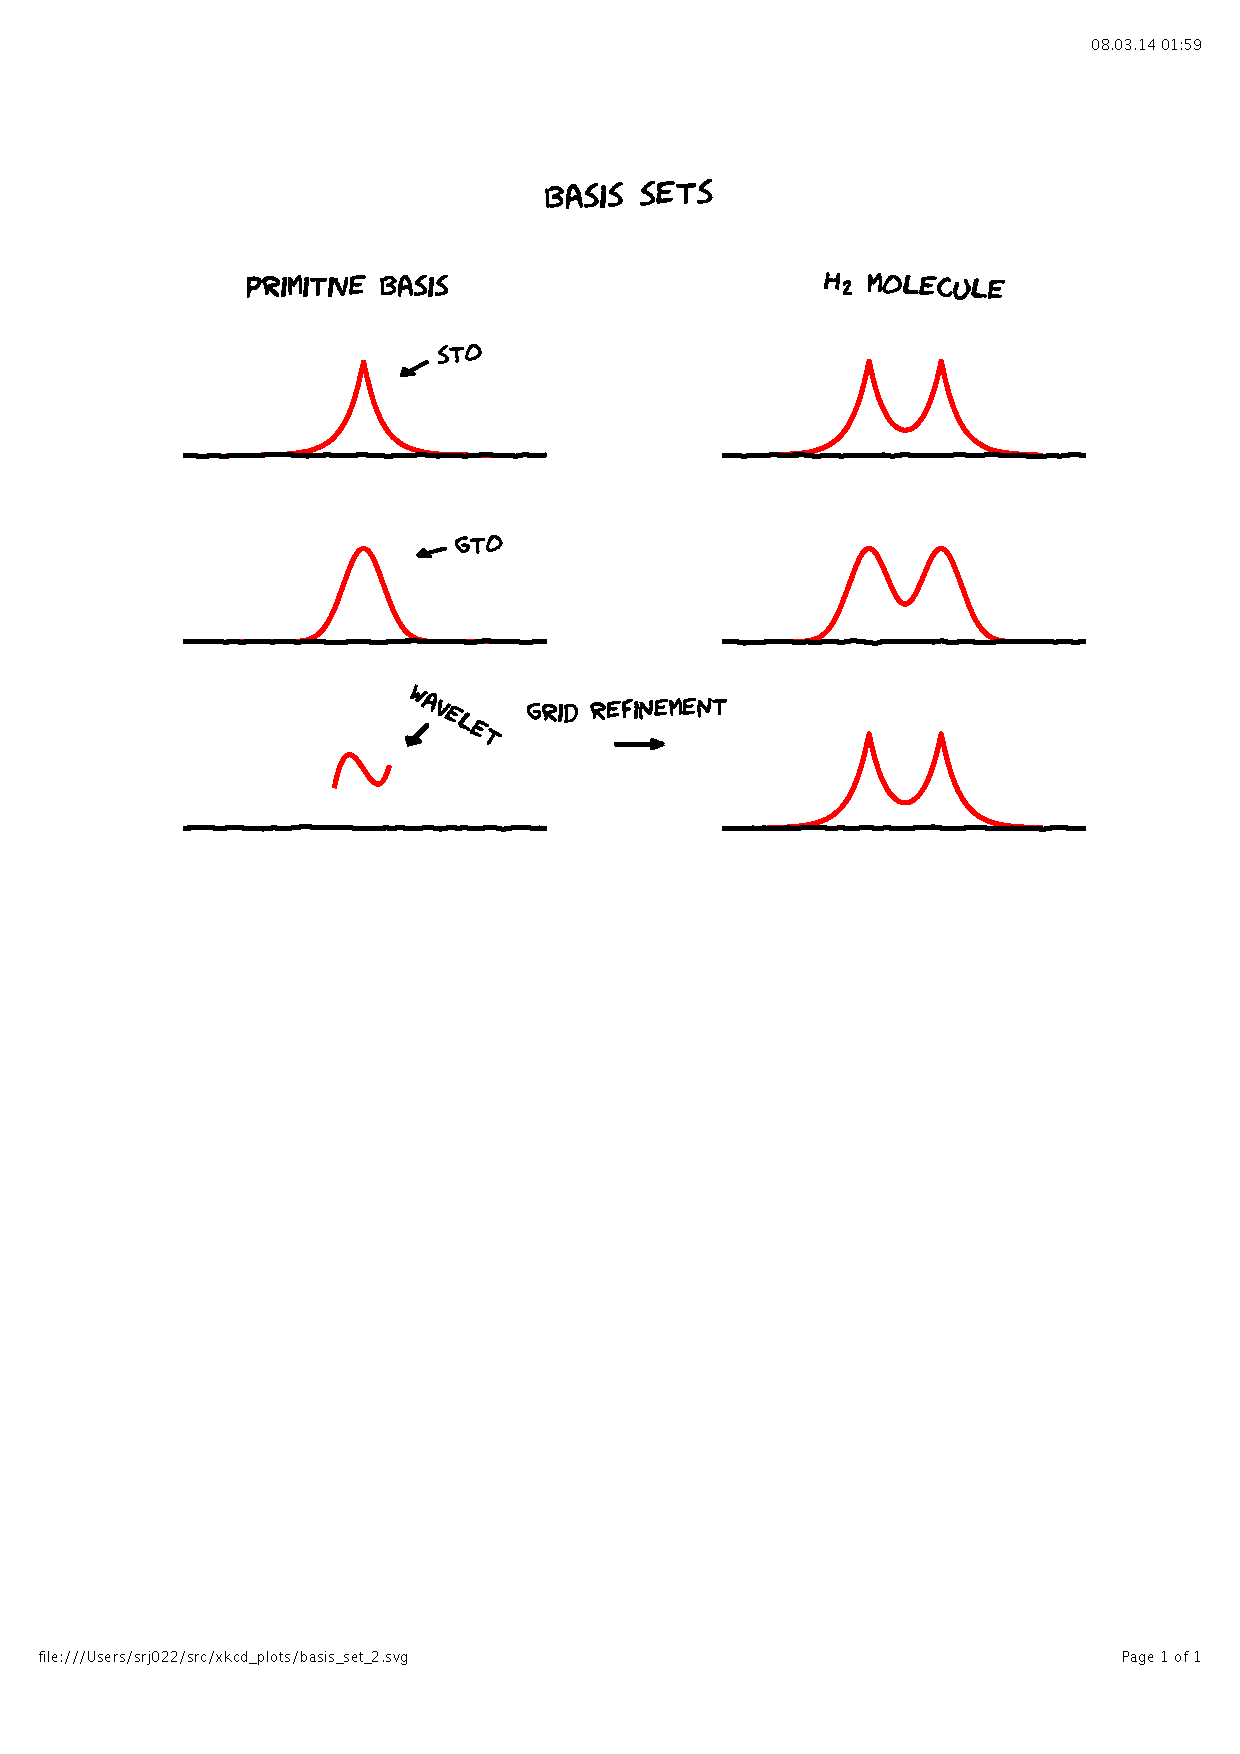
\includegraphics[scale=0.6, clip, viewport = 50 435 550 515]{figures/basis_set_2.pdf}}
    \end{center}
\end{frame}

\begin{frame}
  \frametitle{Roothaan-Hall equations}
  \centering
  \textbf{Kohn-Sham/Hartree-Fock equations}
  \begin{equation}
    \fockOper \orbital_i(r) = \epsilon_i \orbital_i(r)
  \end{equation}

  \vspace{5mm}

  \begin{itemize}
    \item MOs are usually expressed in a Linear Combination of Atomic Orbitals (LCAO) basis:
        \begin{equation}
            \orbital_i(r) = \sum_p C_{ip}\chi_p(r)
        \end{equation}
    \item Leads to the Roothaan-Hall matrix equations:
        \begin{equation}
            \bs{F}\bs{C} = \bs{S}\bs{C}\bs{\epsilon}
        \end{equation}
    \item Iterative solution to find a \emph{self-consistent} coefficient matrix
    \vspace{5mm}
    \item Can we do the same with MWs?
  \end{itemize}
\end{frame}

